\documentclass[convert={density=300,size=1080x800,outext=.png}]{standalone}
\usepackage{tkz-graph}
\usetikzlibrary{arrows,positioning,snakes,shapes,shapes.multipart,patterns,mindmap,shadows}
\usepackage{xcolor}
\usepackage{helvet}
\renewcommand{\familydefault}{\sfdefault}


\begin{document}

\footnotesize
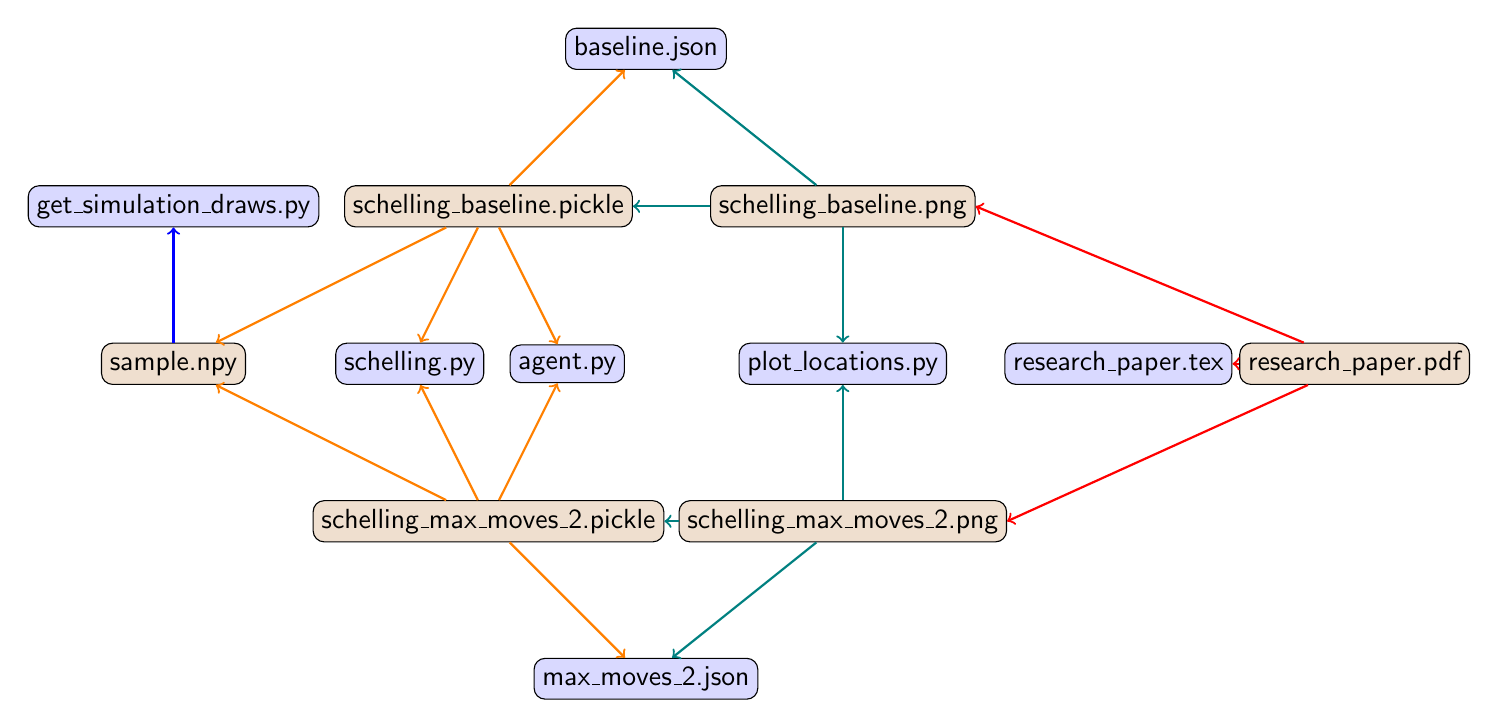
\begin{tikzpicture}[every node/.style={
    rectangle,
    rounded corners,
    inner sep=3pt,
    draw,
    fill=brown!25
}]
    \node (get_simulation_draws_py) [fill=blue!15, shift={(-4, 2)}]
    {
        get\_simulation\_draws.py
    };
    \node (sample_npy) [shift={(-4, 0)}]
    {
        sample.npy
    };
    \node (schelling_py) [fill=blue!15, shift={(-1, 0)}]
    {
        schelling.py
    };
    \node (agent_py) [fill=blue!15, shift={(1, 0)}]
    {
        agent.py
    };
    \node (baseline_json) [fill=blue!15, shift={(2, 4)}]
    {
        baseline.json
    };
    \node (max_moves_2_json) [fill=blue!15, shift={(2, -4)}]
    {
        max\_moves\_2.json
    };
    \node (schelling_baseline_pickle) [shift={(0, 2)}]
    {
        schelling\_baseline.pickle
    };
    \node (schelling_max_moves_2_pickle) [shift={(0, -2)}]
    {
        schelling\_max\_moves\_2.pickle
    };
    \node (plot_locations_py) [fill=blue!15, shift={(4.5, 0)}]
    {
        plot\_locations.py
    };
    \node (schelling_baseline_png) [shift={(4.5, 2)}]
    {
        schelling\_baseline.png
    };
    \node (schelling_max_moves_2_png) [shift={(4.5, -2)}]
    {
        schelling\_max\_moves\_2.png
    };
    \node (research_paper_tex) [fill=blue!15, shift={(8, 0)}]
    {
        research\_paper.tex
    };
    \node (research_paper_pdf) [shift={(11, 0)}]
    {
        research\_paper.pdf
    };
    \draw[->, blue, thick] (sample_npy) to (get_simulation_draws_py);
    \draw[->, orange, thick] (schelling_baseline_pickle) to (sample_npy);
    \draw[->, orange, thick] (schelling_baseline_pickle) to (schelling_py);
    \draw[->, orange, thick] (schelling_baseline_pickle) to (agent_py);    
    \draw[->, orange, thick] (schelling_baseline_pickle) to (baseline_json);
    \draw[->, orange, thick] (schelling_max_moves_2_pickle) to (sample_npy);
    \draw[->, orange, thick] (schelling_max_moves_2_pickle) to (schelling_py);
    \draw[->, orange, thick] (schelling_max_moves_2_pickle) to (agent_py);    
    \draw[->, orange, thick] (schelling_max_moves_2_pickle) to (max_moves_2_json);
    \draw[->, teal, thick] (schelling_baseline_png) to (schelling_baseline_pickle);
    \draw[->, teal, thick] (schelling_baseline_png) to (plot_locations_py);
    \draw[->, teal, thick] (schelling_baseline_png) to (baseline_json);
    \draw[->, teal, thick] (schelling_max_moves_2_png) to (schelling_max_moves_2_pickle);
    \draw[->, teal, thick] (schelling_max_moves_2_png) to (plot_locations_py);
    \draw[->, teal, thick] (schelling_max_moves_2_png) to (max_moves_2_json);
    \draw[->, red, thick] (research_paper_pdf) to (research_paper_tex);
    \draw[->, red, thick] (research_paper_pdf) to (schelling_baseline_png.east);
    \draw[->, red, thick] (research_paper_pdf) to (schelling_max_moves_2_png.east);
\end{tikzpicture}

\end{document}